\chapter{Introduction}
\label{chap:intro}

\graphicspath{{Chapter1/figures/}}

\section{Background}
\lettrine{S}{ensemaking} reflects how we make sense of the world so that we can take further actions~\cite{Snowden2005}. It is a motivated and continuous effort to understand the relationships among people, places and events around us~\cite{Klein2006a}. More specifically, sensemaking is described as the process of collecting, representing and organizing complex information sets based on a particular problem in such a way that can help us understand the problem better and make sense of it more effectively~\cite{Russell2008}. Sensemaking can be some activity that happens everyday such as finding a smartwatch that suits our needs, which may involve searching for different models, learning unfamiliar jargons, and considering pros and cons between those identified models. More rigorously, intelligence analysis~\cite{Heuer1999} can be considered as a complex sensemaking task, in which analysts need to examine thousands of reports to establish deep understanding of particular organizations before identifying potential threats from them. To effectively make sense of problems, people need to digest a large amount of data: tens of smartwatch models, thousands of documents, or a much bigger scale. The data around the world has been produced more rapidly than ever before, with major sources including sensors, machine logs, public websites and social media. In a single day, 50 million photos are uploaded on Instagram, 500 million tweets are sent on Twitter and 3.5 billion searches are performed on Google~\footnote{\url{http://www.internetlivestats.com/}}. This data deluge could help us find more relevant information to our problems; however, it also poses a huge challenge in making sense of such a vast amount of data.

\emph{Visualization} can help people solve problems more effectively through visual representations of datasets~\cite{Munzner2014}. Visual designs can display a large amount of data in a way that quickly reveals hidden patterns. Interaction allows people to further investigate the visualized data in more detail and explore the relationship between identified patterns. Automated techniques in information retrieval and data mining can help speed up the sensemaking process. For instance, named-entity recognition techniques~\cite{Nadeau2007} can automatically identify entities from text and classify them into predefined categories such as persons, organizations and locations. This automation saves analysts a considerable amount of time in their common tasks such as findings all reports mentioning a particular person. \emph{Visual analytics} combines such automated analysis techniques and interactive visualizations to effectively make sense of very large and complex datasets~\cite{Keim2010}.

Research in visual analytics focuses on helping people reveal hidden patterns in the data; however, sensemaking requires support beyond that. After identifying interesting patterns, analysts may need to connect these individual ones to explore the relationships between them, generate potential hypotheses explaining those relationships, and find ways to verify them. Unfortunately, people with limited capacity of working memory cannot hold all of these artifacts simultaneously~\cite{Heuer1999}. They may forget previous findings and relations between them, or remember but fail to retrieve the information needed. They may also forget how those findings were derived, making it more difficult to find similar information. Especially for long and interrupted analysis sessions, people often get lost in the problem space: they are unable to examine their progresses, unable to synthesize their discoveries, and unable to decide the next step effectively.

\emph{Analytic provenance} has the potential to address these problems. It is a subfield of  visual analytics, focusing on understanding a user's reasoning process through the study of their interactions with the computer system that supports sensemaking~\cite{North2011}. Analytic provenance captures both the interactive data exploration process and the accompanied reasoning process during sensemaking~\cite{Xu2015}, releasing analysts from a burden of keeping track of their discoveries. The provenance data then can be visualized to provide different types of support to the users, focusing on post hoc applications of provenance data such as replication, presentation and meta-analysis~\cite{Ragan2016}. Others aim to facilitate sensemaking but are limited in recall of the past process and recovery of performed actions~\cite{Heer2008}. Those provenance visualizations are not specifically designed to support the ongoing, iterative and dynamic sensemaking process, which will be addressed in this thesis.

\section{Research Problem and Approach}

The central research problem of this thesis is
\begin{center}
	\strong{How can we design interactive visualizations\\ of analytic provenance data to support sensemaking?}
\end{center}

To approach the research problem, we propose a cyclic process model, in which analytic provenance can be used to support sensemaking as illustrated in \autoref{fig:intro-workflow}. The process starts with a \emph{user} employing a \emph{sensemaking system} to solve a problem. The sensemaking system could be any computer-based applications, such as a simple visualization tool, a complex visual analytics system and a standard web browser. During the sensemaking process, both the performed low-level actions (e.g., sort, filter and zoom) and the produced high-level reasoning artifacts (e.g., findings, assumptions and hypotheses) are captured, referred to as \emph{provenance data}. This provenance data should be visualized in a way that can provide support back to the ongoing sensemaking process. The user can interact with both the sensemaking system and the \emph{provenance visualization} to solve the sensemaking problem. These two components should communicate with each other to facilitate the interplay between the user and these two. The provenance visualization here acts as a black box and can be implemented using the classic visualization pipeline~\cite{Card1999}.

\begin{figure}[h]
	\centering
	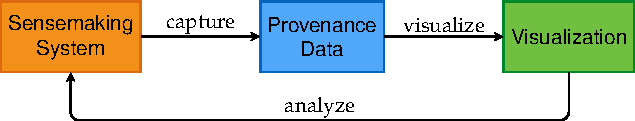
\includegraphics{workflow}
	\caption[A cyclic sensemaking-support model through analytic provenance]{A cyclic process model of supporting sensemaking through analytic provenance. While using a sensemaking system to solve a problem, both the interaction and reasoning performed by the user are \emph{captured} and \emph{visualized} to provide \emph{support} back to the sensemaking process. The sensemaking system can be any computer-based applications such as visual analytics systems and web browsers. The two-way dashed line indicates the communication between the provenance visualization and the sensemaking system to provide sensemaking support. As a result, the user interacts with both the sensemaking system and the provenance visualization to make sense of his or her problem.}
	\label{fig:intro-workflow}
\end{figure}

\subsection{Data and Task Characterization}
In this model, the provenance visualization takes the provenance data as input and the sensemaking support it provides as output. Therefore, it is essential to discuss in the scope of this thesis: what \emph{data} will be visualized and what \emph{tasks} will be supported?

\subsubsection{What data will be visualized?}
Data of analytic provenance can be categorized using a multiple semantic layer model~\cite{Gotz2009}. Low-level actions such as ``\emph{sorting} the bar chart'' or ``\emph{searching} for a keyword'' can be captured automatically but contain little semantics. Higher level reasoning artifacts such as an interesting insight or a potential hypothesis contain richer semantics but capturing such information is much more challenging because they are often a user's inside thoughts. A common method to capture such high semantic provenance data is to allow users to externalize their thinking through note taking or annotation. This thesis will visualize both these two semantic levels of provenance data, focusing on the following characteristics.

\paragraph{Time}
This is an inherent attribute of provenance data. Every provenance data item can be associated with a \emph{timestamp} when it is collected or when it is created. For example, it could represent the time when a sorting action was performed. Or in a more sophisticated and indirect way, it could indicate the time when a suspicious event described in a user's note happened.

\paragraph{Group}
Besides the temporal aspect that can be captured automatically, \emph{grouping} relationship of the raw collected data could be useful for complex sensemaking tasks. Such information could come from a manual assignment, in which a user groups related data together based on their own assessment. It could also come from an automatic process such as a topic modeling technique~\cite{Blei2003}, which can identify notable topics discussed in user notes.

\paragraph{Link}
Another type of data attribute that will be considered in this thesis is \emph{pair-wise link}, showing a direct relationship between two provenance data items. For example, it could represent an origin relationship between two web pages (page $A$ is opened from page $B$). More complicated, it may also be used to indicate a reasoning relationship: a particular event is the reason that leads to a suspicious event.

\subsubsection{What tasks will be supported?}
The tasks described here are not specific visualization tasks that can be categorized by existing taxonomies~\cite{Amar2005, Yi2007, Brehmer2013}. We refer tasks to supporting users in exploring more general types of relationship hidden in the sensemaking problem.

\paragraph{Temporal Relationship}
The \emph{time} attribute of provenance data suggests the task it can support the users: exploring \emph{temporal} relationship. Timestamped low-level actions can help a user recall of his or her sensemaking process: what the user has done, in which order, and at exactly what time? At a higher semantic level, a visualization of user notes about timestamped events can help connect individual pieces of insight together to produce an interesting chronological pattern in the sensemaking problem. Exploring additional grouping information of provenance data could also lead to a more complex temporal relationship.

\paragraph{Reasoning Relationship}
After understanding how things happened in a particular order, it is essential to investigate the \emph{rationale} driving them happened in that way; i.e., advancing from \emph{when} to \emph{why}. Such knowledge is valuable for building effective tools to support the users in making sense of their problems. Considering the sensemaking task as ``selecting a smartwatch'', reasoning relationships can include the rationale behind the smartwatch choice, the strategy in approaching the task and the steps taken to implement that strategy. Additional grouping and linking attributes of provenance data could also help explore more complex reasoning relationships.

\begin{figure}[tb]
	\centering
	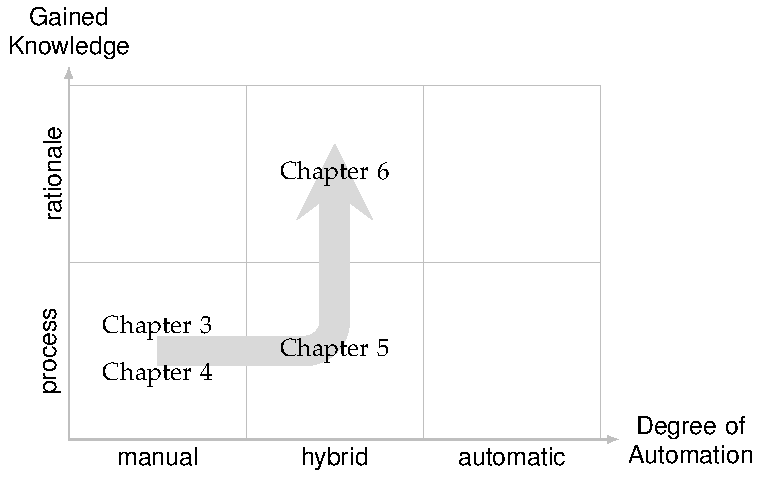
\includegraphics{work}
	\caption[Four research questions]{Four research questions (RQ1 -- RQ4). The research problem is split into the four questions by the data that will be visualized and the task that will be supported in each research question. The horizontal axis represents different types of relationship in sensemaking and the vertical axis represents the complexity involved in the relationship. The cells define the scope of the research questions: the relationship type, its complexity and the characteristics of provenance data involved. For example, Research Question 4 explores complex reasoning relationships in sensemaking based on timestamped provenance data, and additional groupings and pair-wise links between data items.}
	\label{fig:intro-work}
\end{figure}

\subsection{Research Questions}
\label{intro:questions}
To address the research problem, we break it down into four research questions based on the previous \emph{data} (time, group and link) and \emph{task} (temporal and reasoning relationships) characterization. \autoref{fig:intro-work} shows how the research questions relate to the two characterizing dimensions. We believe that analytic provenance can benefit sensemaking in many different application domains. Therefore, the entire thesis does not focus on a single one. Instead, each research question will try to target a different domain to demonstrate the wide application of analytic provenance. For each research question, besides the data and task, we describe the domain and context we want to focus by elaborating on the components of the sensemaking-support model proposed earlier (\autoref{fig:intro-workflow}). Who are the users? Which problems do they want to solve? Which tools do they use to solve those tasks?

\subsubsection*{1. How to design interactive visualizations of \strong{timestamped provenance data} enabling users to explore \strong{temporal relationships in sensemaking}?}
In this research question, we target sensemaking in \emph{intelligence analysis} -- the original domain that sets the foundation for visual analytics research~\cite{Thomas2005}. A common task in intelligence analysis is to examine thousands of reports to identify potential threats from particular organizations. Many visual analytics systems have been designed to facilitate this analysis~\cite{Wright2006,Stasko2007}. To help manage a large number of discoveries, these systems often allow users to take notes (i.e., high-level provenance data) and visualize the notes based on the time when they were taken. However, these temporal visualizations mainly serve as chronologies to remind what happened rather than specifically designed for the exploration of notes to support the iterative and dynamic nature of sensemaking. The design should help users explore a hidden story and construct narratives rather than simply presenting a known one.

\subsubsection*{2. How to design interactive visualizations that can reveal both \strong{temporal and categorical dimensions of provenance data} and enable users to explore more \strong{complex temporal relationships in sensemaking}?}
As discussed earlier, grouping relationship of provenance data items can be added  to help explore more complex relationships in the sensemaking problem. To the best of our knowledge, no existing visualization techniques are designed to show both temporal and categorical information effectively. Therefore, we aim for a general design of timeline visualization that can apply to multiple domains. We start with the same intelligence analysis domain as in the previous question, then explore the use of our design in other domains.

\subsubsection*{3. How to design interactive visualization tools for \strong{timestamped provenance data} that enables analysts to explore \strong{reasoning relationships in sensemaking} performed by other users?}
This question targets the \emph{sensemaking research} or \emph{qualitative research}~\cite{Adams2008} in general. To explore reasoning relationships of sensemaking, researchers often take a qualitative approach: conduct a user study to observe the process, transcribe screen capture videos and think-aloud recordings, identify recurring patterns in the produced transcript, and eventually abstract the sensemaking process into a general model. Note that two types of people are involved in this research question: the \emph{sensemaking user} who participates in the study and the \emph{sensemaking researcher} who conducts the study to understand the sensemaking process performed by the participant. Currently, such a qualitative research process is highly manual and time-consuming~\cite{Wong2002}. Which steps in that process can be automated or facilitated by analytic provenance? Can analytic provenance data recorded in the study, especially low-level actions, help researchers understand the reasoning relationships of the participant's sensemaking process? Which data should be captured and how can they be visualized to facilitate the analysis?

\subsubsection*{4. How to design interactive visualization tools for \strong{timestamped provenance data} that can incorporate \strong{user-added relations} and enable users to explore more \strong{complex reasoning relationships in sensemaking}?}

This research question targets a widely applicable domain: browser-based online, everyday sensemaking. To make sense of everyday tasks such as selecting a suitable camera, a common approach is to use standard web browsers (simple sensemaking systems) to search for different models and consider their strengths and weaknesses before making a decision. The provenance data includes automatically captured low-level actions as in the previous question. Additionally, users can be offered to contribute rich semantics to the data through manipulation of the visualized provenance. Can such rich provenance data help users explore more complex reasoning relationships and achieve a better sensemaking performance? Does the benefit that users gain outweigh the overload that they put in providing extra information richness?

\subsubsection*{\textbf{Approach to Research Questions}}
We take a user-centered design approach in seeking solutions to all of the research questions. For each question, we elicit the design requirements by conducting a user study with end users and/or drawing from the literature. Visual encoding and interaction are designed to meet those requirements, and the designs are implemented into a working prototype. Finally, an empirical study is conducted to explore how the tool is used by target audience to perform target tasks, and to investigate whether and how the tool provides the intended sensemaking support.

\section{Thesis Contributions}
Toward the overall goal of supporting users in their sensemaking processes through the visualizations of provenance data, this thesis contributes:

\paragraph{SchemaLine} A timeline visualization technique that enables users to examine information in chronological order, identify temporal patterns and construct narratives from relevant user notes. It produces a compact but aesthetically pleasing layout allowing users to easily follow the events happening within individual narratives. It also provides a set of fluid interactions supporting users in performing various sensemaking activities described in the Data--Frame model~\cite{Klein2003}. This work is to address Research Question 1 and was published as

\textbf{P. H. Nguyen}, K. Xu, R. Walker, and B. L. W. Wong. SchemaLine: Timeline Visualization for Sensemaking. In \textit{International Conference on Information Visualization}, pages 225--233. IEEE, jul 2014.

\paragraph{TimeSets} A timeline visualization technique that enables users to explore complex temporal relationships by effectively representing both temporal and categorical provenance data. It visually groups data elements that share the same group but still preserves their temporal order. TimeSets color codes the backgrounds of the entire groups to distinguish them and uses colored gradient backgrounds for the intersections among those groups. It also adjusts the level of details of each data item dynamically to accommodate more items within a given display estate. This is to address Research Question 2 and was published as

\textbf{P. H. Nguyen}, K. Xu, R. Walker, and B. L. W. Wong. TimeSets: Timeline visualization with set relations. \textit{Information Visualization}, 15(3):253--269, jul 2016.

K. Xu, \textbf{P. H. Nguyen}, and B. Fields. Visual analysis of streaming data with SAVI and SenseMAP. In \textit{IEEE Conference on Visual Analytics Science and Technology}, pages 389--390. IEEE, oct 2014.

\paragraph{SensePath} A visual sensemaking tool that enables researchers to explore reasoning relationships of the sensemaking process effectively and efficiently. It offers an alternative approach in performing transcription and coding (the two time-consuming stages in the qualitative analysis process). In stead of having to transcribe the video, SensePath automatically captures and detects participant's sensemaking actions, and provides multi-linked visualizations to support further analysis. It visualizes provenance data in a timeline that enables researchers to quickly gain an overview of the sensemaking process and identify recurring sensemaking patterns. It also links with a screen capture video to allow researchers to examine  additional context when necessary. To enable researchers to continue working on the subsequent stages of analysis using their normal workflow, SensePath exports its coded transcript in a common format that can be used by other popular qualitative data analysis software packages. Through a small scale user study, SensePath was shown to help qualitative analysts complete transcription and coding with a comparable quality with traditional analysis and finish within less time. This is to address Research Question 3 and was published as

\textbf{P. H. Nguyen}, K. Xu, A. Wheat, B. L. W. Wong, S. Attfield, and B. Fields. SensePath: Understanding the Sensemaking Process through Analytic Provenance. \textit{IEEE Transactions on Visualization and Computer Graphics}, 22(1):41--50, jan 2016.

\paragraph{SenseMap} A visual sensemaking tool that enables users to explore complex reasoning relationships of sensemaking. It automatically captures and detects sensemaking actions and relationships between these actions before visualizing both of them in a branching history tree. This allows users to examine the reasoning relationships between the actions they performed, remind them of what have been done earlier, and potentially suggest the next step. To help explain more complex relationship, SenseMap provides an intuitive interface for users to assign additional meaning to the automatically collected data by spatially grouping actions or adding reasoning links between them. It also allows users to communicate their analysis results at different levels of granularity including a big picture of user-organized findings, a more detailed analysis process and raw evidence captured. A user-centered evaluation showed that when participants engaged with the tool and spent effort organizing their analytic provenance data in the visualization views, they were able to produce higher quality sensemaking outcome. This is to address Research Question 4 and was published as

\textbf{P. H. Nguyen}, K. Xu, A. Bardill, S. Betul, K. Herd, and B. L. W. Wong. SenseMap: Supporting Browser-based Online Sensemaking through Analytic Provenance. In \textit{IEEE Conference on Visual Analytics Science and Technology}, pages 91--100, oct 2016.
\\

\noindent Besides the main contributions described in this thesis, I also coauthored the following articles related to analytic provenance for sensemaking.

\begin{itemize}
	\item I contributed to the discussion and the design of a framework for provenance in human terrain analysis, and the work was published as

	\quad R. Walker, A. Slingsby, J. Dykes, K. Xu, J. Wood, \textbf{P. H. Nguyen}, D. Stephens, B. L. W. Wong, and Y. Zheng. An extensible framework for provenance in human terrain visual analytics. \textit{IEEE Transactions on Visualization and Computer Graphics}, 19(12):2139--2148, dec 2013.

	\item I contributed to the organization of a IEEE VIS workshop on provenance for sensemaking. The discussion at the workshop was published as

	\quad K. Xu, S. Attfield, T. J. Jankun-Kelly, A. Wheat, \textbf{P. H. Nguyen}, and N. Selvaraj. Analytic provenance for sensemaking: a research agenda. IEEE Computer Graphics and Applications, 35(3):56--64, jan 2015.
\end{itemize}

\section{Thesis Outline}
The remainder of this thesis is organized as follows.

First, \autoref{chap:review} reviews the core work in sensemaking, visualization and visual analytics. It then emphasizes the visualization of analytic provenance data for supporting sensemaking.

\autoref{chap:schemaline} discusses the SchemaLine timeline visualization enabling users to explore temporal relationships of sensemaking -- addressing Research Question 1.

\autoref{chap:timesets} extends \autoref{chap:schemaline} to present the TimeSets visualization technique that can effectively show both temporal and categorical provenance data to reveal complex temporal relationships of sensemaking -- addressing Research Question 2.

\autoref{chap:sensepath} discusses the SensePath visualization tool that can exploit timestamped provenance data, enabling users to explore reasoning relationships of sensemaking -- addressing Research Question 3.

\autoref{chap:sensemap} describes the SenseMap visualization tool that incorporates additional grouping and linking attributes with provenance data enabling users to explore complex reasoning relationships of sensemaking -- addressing Research Question 4.

Finally, \autoref{chap:conclusion} concludes the thesis with a discussion on its contributions and future research directions triggered from this work.